%
% NOTE -- ONLY EDIT THE .Rnw FILE!!!  The .tex file is
% likely to be overwritten.
%
%\VignetteDepends{RGtk, gtkDevice, graph, Rgraphviz}
%\VignetteKeywords{Model, View, Controller}
%\VignettePackage{MVCClass}
%\VignetteIndexEntry{MVCClass}

\documentclass[11pt]{article}


\usepackage{amsmath,pstricks}
\usepackage[authoryear,round]{natbib}
\usepackage{hyperref}
\usepackage{times}
\usepackage{comment}
\usepackage{epsfig}
\usepackage{graphics}
\usepackage{graphicx}


\textwidth=6.2in
\textheight=8.5in
%\parskip=.3cm
\oddsidemargin=.1in
\evensidemargin=.1in
\headheight=-.3in

\newcommand{\scscst}{\scriptscriptstyle}
\newcommand{\scst}{\scriptstyle}

\newcommand{\Rfunction}[1]{{\texttt{#1}}}
\newcommand{\Robject}[1]{{\texttt{#1}}}
\newcommand{\Rpackage}[1]{{\textit{#1}}}


\bibliographystyle{plainnat}

\title{Model-View-Controller Package}
\author{Elizabeth Whalen}
\date{November 11, 2005}

\usepackage{/home/ewhalen/sw/R-devel/lib/R/share/texmf/Sweave}
\begin{document}
\maketitle

\section{Overview}\label{Sec:Overview}

The purpose of the \Rpackage{MVCClass} package is to provide the definitions of
classes and generic functions that will be used by other packages to create 
model-view-controller applications.  Currently, the packages that use the 
\Rpackage{MVCClass} package are \Rpackage{iSPlot} and \Rpackage{iSNetwork}.  
Both packages use the definitions from \Rpackage{MVCClass} to create linked, 
interactive views of data.

\section{MVC Class}\label{Sec:MVC}

The \Robject{MVC} class represents a model-view-controller object.  Basically, 
this class will bind the model with its views and its controller so that 
an object of this class can be created each time there is a new data set 
(model).  Thus, there is a one-to-one relationship between a MVC object and
a model object.  Because of this relationship, the
MVC object and the model object are identified by the same name,
which is stored in the modelName slot of the model object (see Section 
\ref{Sec:Model}).  The figure below 
shows the class definition for \Robject{MVC}. 

\begin{figure}[ht]
  \begin{center}
    \scalebox{0.3}{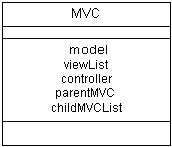
\includegraphics{MVCClass.jpg}}
    \caption{ The MVC Class. }
    \label{Fig:MVCClass}
  \end{center}
\end{figure}

The \Robject{MVC} class has five slots which are model, viewList, controller, 
parentMVC, and childMVCList.  The
model slot stores the model object, the viewList slot is a list of the view
objects for this model, the controller slot is an environment that stores
information for this MVC, the parentMVC slot is the name of the parent model
(MVC), and the childMVCList slot is a list of the children models
(MVCs).  Note that model and MVC objects use the same name so the
parentMVC slot refers to both the name of the model and the name of the
MVC.  Similarly, for the childMVCList slot, the names in the list
refer to both the name of the model and the name of the MVC.

Thus, the \Robject{MVC} class not only binds the model, view, and controller
objects together, but MVC objects can be related to each through a 
parent-child (tree) hierarchy because of the slots, parentMVC and 
childMVCList. 
These two slots also show that a MVC object can have at most one parent MVC and
can have as many children MVCs as it wants. 

\section{Model Classes}\label{Sec:Model}

The model class is responsible for storing and updating the data.  These two
functions are reflected in Figure \ref{Fig:Model}, which shows the inheritance
structure for the model classes.  Here the virtual class,
\Robject{gModel}, has the slots modelData, linkData, virtualData, and
modelName.  These four slots are common information that all models will
need.  The modelData slot is the data set for this model, the linkData slot is
a list of two functions, \Rfunction{linkToParent} and \Rfunction{linkToChild},
which link this model to its parent and child models, respectively (see Section
\ref{Sec:MVC}), the virtualData slot is data pertaining to the views
that needs to be stored with the model so that it can be shown in all views of
this model, and the modelName slot is the name of the model. 

\begin{figure}[ht]
  \begin{center}
    \scalebox{0.7}{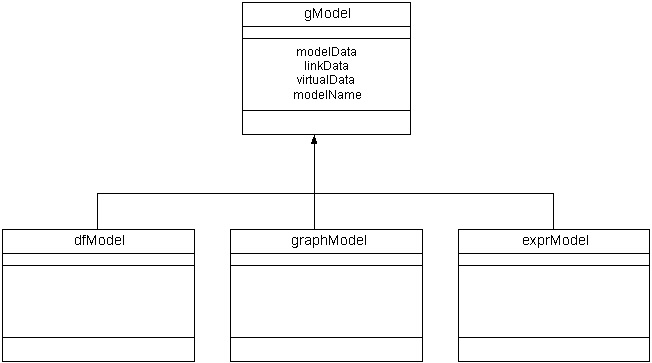
\includegraphics{VigModelClass.jpg}}
    \caption{ Inheritance for Model Objects. }
    \label{Fig:Model}
  \end{center}
\end{figure}

For specific model classes, there are \Robject{dfModel}, \Robject{graphModel},
and \Robject{exprModel}.  The \Robject{dfModel} class represents a model where
the modelData has class data frame (or matrix), the \Robject{graphModel} class
represents a model where the modelData has class graph, and the
\Robject{exprModel} class represents a model where the modelData has class
exprSet. 

As mentioned previously, the model classes are also responsible for updating
the data so a generic function \Rfunction{updateModel} has also been 
defined.  The \Rfunction{updateModel} methods will be defined in packages that 
use this package (i.e. the methods will be defined in \Rpackage{iSNetwork} and 
\Rpackage{iSPlot}).

\section{View Classes}\label{Sec:View}

The view classes represent the visual depictions of the model.  All views will
need to store some common information and respond to certain events through
methods.  This consideration led to an object model where the different view
classes inherit from a view virtual class, called \Robject{genView}.  The
object model for the view classes is shown in Figure \ref{Fig:View}.

\begin{figure}[ht]
  \begin{center}
    \scalebox{0.7}{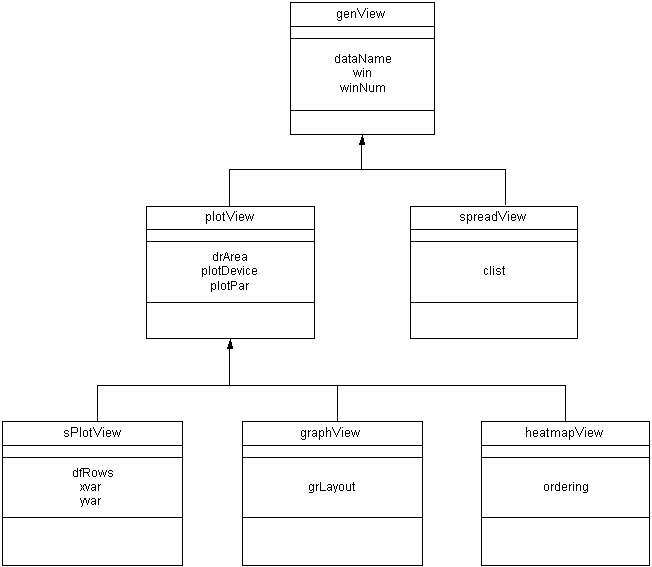
\includegraphics{VigViewClass.jpg}}
    \caption{ Inheritance for View Objects. }
    \label{Fig:View}
  \end{center}
\end{figure}

The \Robject{genView} class has three slots, dataName, win, and winNum.
dataName is the name of the model that the view displays, win is the Gtk
window object that holds the view, and winNum is the number of the window so
that the window can be identified in the GUI that other packages create.  All 
views will need to know these three pieces of information so \Robject{genView} 
will bind the view classes together. 

As for specific view classes, the \Robject{spreadView} class will represent a
spreadsheet view of the data.  This view will only make sense for models that
are a two dimensional data structure, such as a matrix or a data frame.  The
information needed for this view is stored in the slot, clist, which is the
Gtk spreadsheet object.

When creating a plot of a data set, there is a general class, called
\Robject{plotView}, that has the slots, plotDevice, plotPar, and drArea, which
store the device number of the plot, the plotting parameters, and the Gtk
drawing area object, respectively.  This class is not intended to have any
objects as it just represents a general plot.  The plot classes that can have
objects are the specific plot classes, \Robject{sPlotView},
\Robject{graphView}, and \Robject{heatmapView}, which inherit from the
\Robject{plotView} class.  

The \Robject{sPlotView} class represents a scatterplot view and it has the
extra slots, dfRows, colx, and coly, where dfRows are the row names from the
model that are shown in the plot, colx is the column name from the model that
is shown as the x variable in the plot, and coly is the column name from the
model that is shown as the y variable in the plot.  The \Robject{graphView}
class represents a graph plot view and it contains no extra slots besides
those in the \Robject{plotView} class.  The \Robject{heatmapView} represents a
heatmap view of the data and it contains the slot, ordering, which is a list
that is returned from the \Rfunction{heatmap} function to give information
about the dendrogram ordering.  Note that some of these views are only
applicable for certain model types. For example, the \Robject{graphView} class
will only make sense for a view of a graph object, which would be stored in the
\Robject{graphModel} class. 

Several generic functions have been defined that refer to operations 
performed on views.  These generic functions are \Rfunction{motionEvent}, 
\Rfunction{clickEvent}, \Rfunction{updateView}, and \Rfunction{redrawView}.  
Methods for these generic 
functions will be defined in packages that use this package (in 
\Rpackage{iSPlot} and \Rpackage{iSNetwork}).  When these methods are defined, 
the \Rfunction{motionEvent} method will be used to respond to a mouse over 
event on a view, the \Rfunction{clickEvent} method will be used to respond to 
a click event over a view, the \Rfunction{updateView} method will be used to 
update only a portion of the view, and the \Rfunction{redrawView} method will 
be used to completely redraw the view.

\section{Message Classes}\label{Sec:Message}

The message classes are intended to provide communication between different
components of the MVC design, such as when the model changes a message needs to
be sent to the views to let them know that they should be updated.  This
communication between the model, view and controller is crucial for the pieces
to work together and yet, still be independent of each other. 

The object model for the message classes was derived from the idea that all
messages must have certain methods in common, such as \Rfunction{initialize}
and \Rfunction{handleMessage}, because all messages must be created and
handled in some manner so that the message is read and acted upon.  Also,
since messages are sent when something has changed, either through addition,
alteration, or deletion, the message classes reflect only certain operations.
These common purposes for the messages allow the message object model to be
constructed, and this model is shown in Figure \ref{Fig:Mess}.

\begin{figure}[ht]
  \begin{center}
    \scalebox{0.7}{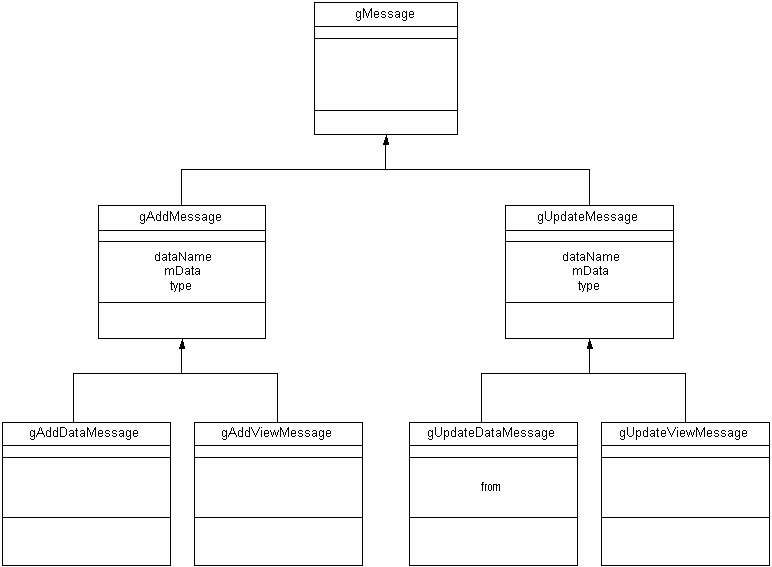
\includegraphics{VigMessageClass.jpg}}
    \caption{ Inheritance for Message Objects. }
    \label{Fig:Mess}
  \end{center}
\end{figure}

The above figure shows the inheritance structure for message objects that can 
be passed within one MVC object and a later figure in this section will show 
the inheritance structure for messages objects that can be passed between MVC 
objects.

As with the view classes, the top message class, \Robject{gMessage}, is a
virtual class.  It contains no slots and its purpose is to bind the other
message classes together.

Currently, there are two types of messages for messaging within a model, view,
controller object: an add and an update message.  Both the add message,
\Robject{gAddMessage}, and the update message, \Robject{gUpdateMessage},
contain three slots, dataName, mData, and type.  dataName is the character
string that gives the name of the model, mData is a list of data needed to
perform the addition or alteration operation, and type is a character string
that gives the type of addition or alteration to perform.  Although
\Robject{gAddMessage} and \Robject{gUpdateMessage} are not virtual classes, it
is not intended to create objects of these classes.

Since adding a view requires different information and methods from adding a
model (and similarly with updating views versus models), it makes sense to
have two separate message classes for these operations.  Thus, when messages
are sent between components, they are from one of the following classes:
\Robject{gAddDataMessage}, \Robject{gAddViewMessage},
\Robject{gUpdateDataMessage}, and \Robject{gUpdateViewMessage}.  As shown in
Figure \ref{Fig:Mess}, the \Robject{gAddDataMessage} and
\Robject{gAddViewMessage} classes inherit from the \Robject{gAddMessage}
class, and the \Robject{gUpdateDataMessage} and \Robject{gUpdateViewMessage}
classes inherit from the \Robject{gUpdateMessage} class. 

The \Robject{gAddDataMessage} class represents a message to add a model and a
MVC object because whenever a model is added, a MVC object is also added that
contains this model.  The \Robject{gAddViewMessage} class represents a message
to create a view.  

The \Robject{gUpdateDataMessage} class represents a message to update
a model.  This message is crucial for linking because it is responsible for
ensuring that once a model has been updated this information must propagate to
any views of the model and this information must also be passed along to any
other MVC object that is related to this model.  Because this information gets
passed to other MVC objects, this message also has one new slot, from, in 
addition to
the slots it inherits from \Robject{gUpdateMessage}.  The from slot is the
name of the model that the update data message came from.  This slot is
necessary because the update data message can come from one of two sources:
the message can occur because of user interaction with a view
of this model or the message may occur because a different model that is
linked to this model has been updated.  So the update data message may come
from within this MVC object or it may come from a different MVC object that
has changed its model and is related to this MVC object.  
Information on passing messages between MVC
objects will be given later in this section.  Finally, the
\Robject{gUpdateViewMessage} class represents a message to update a view.

Message classes have also been defined to pass information between MVC objects.
The two main types of messages, the add and update messages, will also be used 
here.  The inheritance structure for messages passed between MVC objects is 
shown in the figure below.
 
\clearpage

\begin{figure}[ht]
  \begin{center}
    \scalebox{0.7}{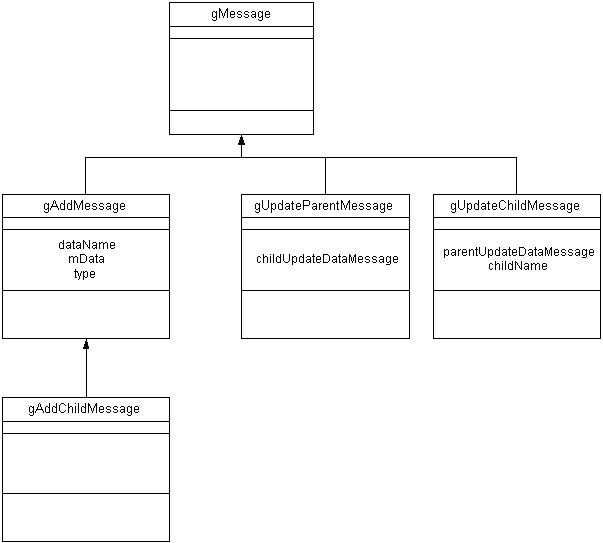
\includegraphics{VigMessageClass2.jpg}}
    \caption{ Inheritance for Message Classes that are Passed Between MVCs. }
    \label{Fig:BetwMess}
  \end{center}
\end{figure}

The first message class that will be discussed is \Robject{gAddChildMessage}.
A \Robject{gAddChildMessage} object will be very similar to a
\Robject{gAddDataMessage} object because they are both adding a new
model and a new MVC object.  The difference with a \Robject{gAddChildMessage}
object is that it must fill in some extra information to tie this new MVC
object to its parent MVC object.  The \Robject{gAddChildMessage} class
inherits from the \Robject{gAddMessage} class, with the same slots of
dataName, mData, and type.  The dataName slot is the name of the new model (and
new MVC), the mData slot is a list that contains the model data and virtual
data to fill the modelData and virtualData slots, respectively, of the new
model, and the type slot gives the type of the model (currently, the options
are ``exprSet'', ``graph'', or ``data.frame'').  

The next two message classes pertain to updating MVC objects when a parent MVC
or child MVC object has changed.  These classes are
\Robject{gUpdateParentMessage} and \Robject{gUpdateChildMessage} and they both
inherit from the \Robject{gMessage} class, as shown in Figure
\ref{Fig:BetwMess}.  Even though they are both update messages, they do not
inherit from the \Robject{gUpdateMessage} class because the information they
need to contain is a \Robject{gUpdateDataMessage} object.  Thus, the
\Robject{gUpdateParentMessage} class has one slot, childUpdateDataMessage, and
this slot contains the \Robject{gUpdateDataMessage} object that was used to
update the child model.  Similarly, the \Robject{gUpdateChildMessage} class
has two slots, parentUpdateDataMessage and childName, where the
parentUpdateDataMessage slot contains the \Robject{gUpdateDataMessage} object
that was used to update the parent model and the childName slot contains the
name of the child model that is being updated (because a parent MVC can have
more than one child MVC). 

A generic function, \Rfunction{handleMessage}, is defined that will be used to 
read message objects.  Methods for this generic function will be defined in 
packages that use this package (\Rpackage{iSPlot} and \Rpackage{iSNetwork}).

\section{Event-Callback Function Class}\label{Sec:EventFun}

Linking callback functions to events, such as a button click, a mouse movement
or a key press event, is what allows users to have an interactive
environment.  Then when an event happens something will occur in response
depending on the callback function linked to the event.  Now to create a
flexible environment we do not want a callback function that always does the
same thing when an event occurs.  For example, when a left button press event
occurs, we may sometimes want a point to be colored and at other times we may
want a point to be hidden.  To allow this flexibility, a class called
\Robject{gEventFun} was created.  By using this class, users will be able to
change the response to an event.  

The \Robject{gEventFun} class stores all of the information about a potential
callback function.  Having the callback function information stored in an 
object will allow a user to connect events to callback functions.  The class 
definition for \Robject{gEventFun} is shown in the figure below.

\begin{figure}[ht]
  \begin{center}
    \scalebox{0.3}{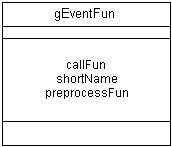
\includegraphics{EventClass.jpg}}
    \caption{ The gEventFun Class. }
    \label{Fig:EventFun}
  \end{center}
\end{figure}

As shown in Fig \ref{Fig:EventFun}, the slots in the \Robject{gEventFun} class
are callFun, shortName, and preprocessFun.  The callFun slot is the name of
the callback function, the shortName slot is a short description of the
function, and the preprocessFun slot is a character vector of all
preprocessing functions that must be called before the callback function.

The callback function that is stored in the callFun slot must take only one
parameter and the class of this parameter will depend on the model class in
the active MVC object.  For example, for a graph model, the
parameter will be of class \Robject{AgNode}, representing a node in the graph.
For a data frame model, the parameter will be of class character, representing
a row in the data frame.

The preprocessing functions that are stored in the preprocessFun slot will
take no parameters.  The purpose of the preprocessing functions is to set some
variables that the callback function will need.  Thus, not all callback
functions will need preprocessing functions and if no preprocessing functions
are needed, then this slot will be NULL.  If the callback function sets the
color of a node in a graph, then a preprocessing function is needed to
determine what color this will be.  So in this example, the preprocessing
function will open a color browser to allow the user to choose what the new
color will be.

\section{Conclusions}\label{Sec:Conc}

The inheritance structure for the classes defined in this package are intended 
to be extensible.  If a user needs a model of a different type that is not 
currently represented, then a new model class can be defined that inherits 
from the \Robject{gModel} virtual class.  Similarly, new view and message 
classes can be created if new views or messages are needed by a user.

As mentioned in Section \ref{Sec:Overview} this package is intended to be a 
behind the scenes package that is used by other packages for its class and 
generic function definitions.  Currently, this package is used by the 
\Rpackage{iSPlot} and \Rpackage{iSNetwork} packages.

\end{document}

